%\newpage
\section{Auswertung}
    \subsection{Bestimmung der Untergrundrate}
        In einem Zeitraum von $T = 327256$s wurden $N_{\text{Start}} = 6543685$ Startsignale und $N_{\text{Stopp}} = 25257$
        Stoppsignale aufgenommen. Damit ergibt sich eine durchschnittliche Rate von:
        \begin{equation*}
            r = \frac{N_{\text{Start}}}{T} = \frac{6543685}{327256} \approx 20,00 \, \frac{\text{Myonen}}{\text{s}}
        \end{equation*}
        Die Wahrscheinlichkeit, dass genau ein weiteres Myon ($k = 1$) in der Suchzeit $T_\text{S} = 10\mu$s nach einem vorherigen Myon ein Signal erzeugt ist poissonverteilt und damit:
        \begin{align*}
            p(k) &= \frac{(T_{\text{S}} \cdot r)^k}{k!} \exp\left(-T_{\text{S}} \cdot r\right) \\[10pt]
            p(1) &= T_{\text{S}} r \cdot \exp\left(-T_{\text{S}}  r\right) \approx 0,02000 \%
        \end{align*}
        Der Untergrund setzt sich aus diesen während einer angefangenen Suchzeit ankommenden Myonen zusammen. Also ist die Anzahl dieser fehlerhaften Signale gegeben durch:
        \begin{equation*}
            N_{\text{fehl}} = p(1) \cdot N_{\text{Start}} \approx 1308
        \end{equation*}
        Für jeden der 225 besetzten Kanäle (gesamt 512 Kanäle) im MCA wäre der Untergrund somit:
        \begin{equation*}
            u_{\text{theo}} \approx 5,81
        \end{equation*}

    \subsection{Justierung der Verzörgerungsleitungen}
        Die Signale aus den Photomultipliern sollten möglichst zeitgleich an der Koinzidenz ankommen. Das heißt, dass die Anzahl der Signale, die die Koinzidenz durchlässt steigt je kleiner der zeitliche Abstand zwischen den beiden ankommenden Signalen ist. Da die beiden Signale nie genau im selben Zeitpunkt ankommen können, hat die Koinzidenz ein kleines Toleranzintervall (die Auflösungszeit), weshalb ein Plateau zu sehen sein müsste, wenn die Counts gegen die Zeitdifferenz auftragen werden.
        
        \begin{figure}[h]
            \centering
            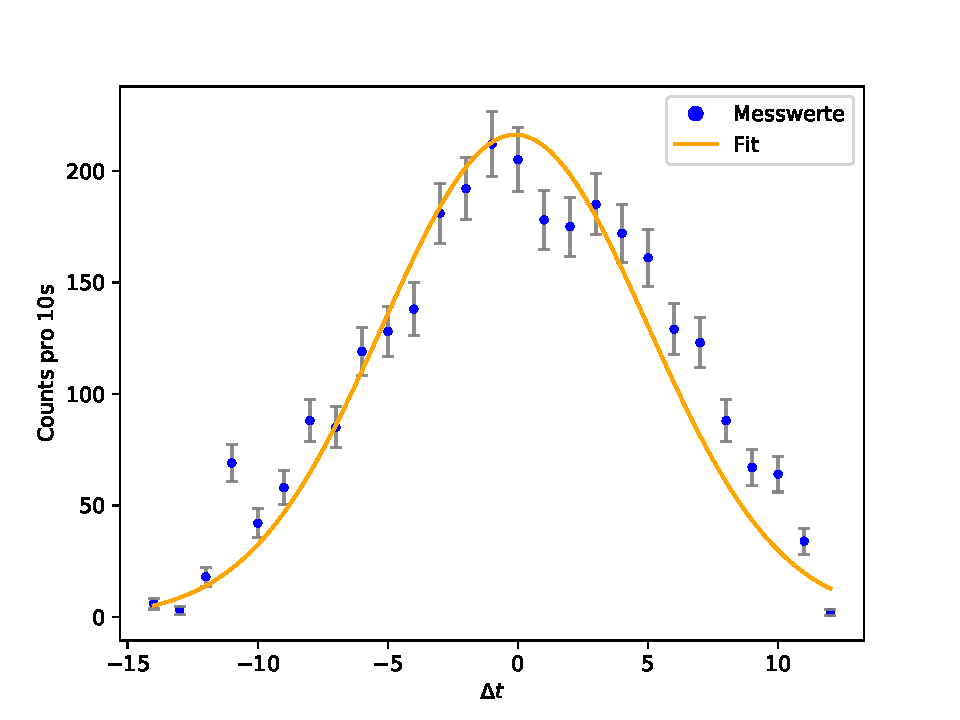
\includegraphics[width = 0.75\textwidth]{plots/Verzoergerung.pdf}
            \caption{Die an der Koinzidenz gemessenen Counts/10s sind gegen die Zeitdifferenz zwischen den beiden Verzörgerungsleitungen aufgetragen.}
            \label{fig:Verzoergerung}
        \end{figure}

        \FloatBarrier

        Es wird eine Gauß-Glocke an die Messwerte gefittet
        \begin{equation*}
            f(x) = a \exp\left(-\frac{\left(x - x_0\right)^2}{2 \sigma^2}\right)
        \end{equation*}
        mit den folgenden Parametern:
        \begin{align*}
            a &= 216,19 \pm 14,21 \\
            x_0 &= (-0,11 \pm 0,29) \, \text{ns} \\
            \sigma &= (-5,08 \pm 0,20) \, \text{ns}
        \end{align*}

        Im Nachfolgenden wurde die Stelle der maximalen Counts als Nullpunkt gewählt und alle darauffolgenden Schritte wurden mit dieser Einstellung der Verzörgerungsleitung durchgeführt.

        \newpage
        \subsection{Kalibration des TAC-MCA}
        Das TAC gibt zu einem gemessenen Zeitintervall proportionale Spannungsamplitude an den MCA weiter, welche dann ihrer Größe nach in Kanäle geordnet werden. Um den Proportionalitätsfaktor zwischen den Amplituden und den Zeitintervallen zu bestimmen werden verschiedene Pulsabstände an einem Doppelimpulsgenerator eingestellt und gegen die Kanäle im MCA aufgetragen. Dadurch wird bestimmt welchem Kanal welcher Zeitabstand zugeordnet ist, bzw. der Propotionalitätsfaktor wird bestimmt.

        \begin{figure}[h]
            \centering
            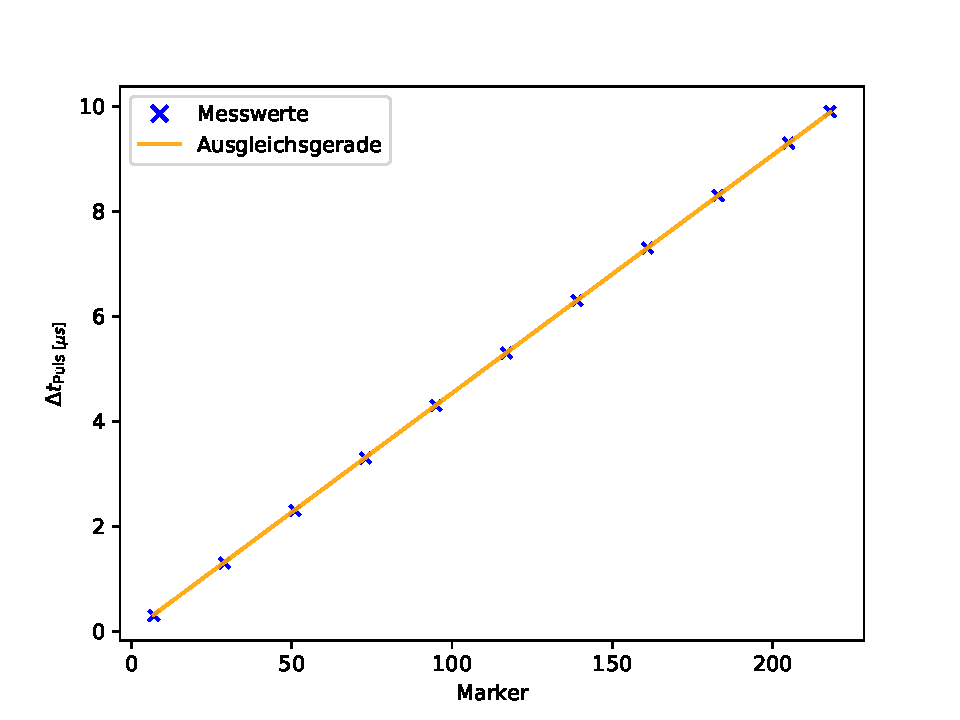
\includegraphics[width = 0.75\textwidth]{plots/Marker_Faktor.pdf}
            \caption{Das eingestellte Zeitintervall zwischen den Pulsen am Doppelimpulsgenerator ist gegen die Kanäle des MCA aufgetragen.}
            \label{fig:Marker_Faktor}
        \end{figure}

        \FloatBarrier

        Durch die Messwerte wird ein linearer Fit gelegt
        \begin{equation*}
            f(x) = m \cdot x
        \end{equation*}
        mit der Steigung:
        \begin{equation*}
            m = (0,045348 \pm 0,000024) \, \mu\text{s}
        \end{equation*}
    
    \newpage
    \subsection{Bestimmung der Lebenszeit}
        \begin{figure}[h]
            \centering
            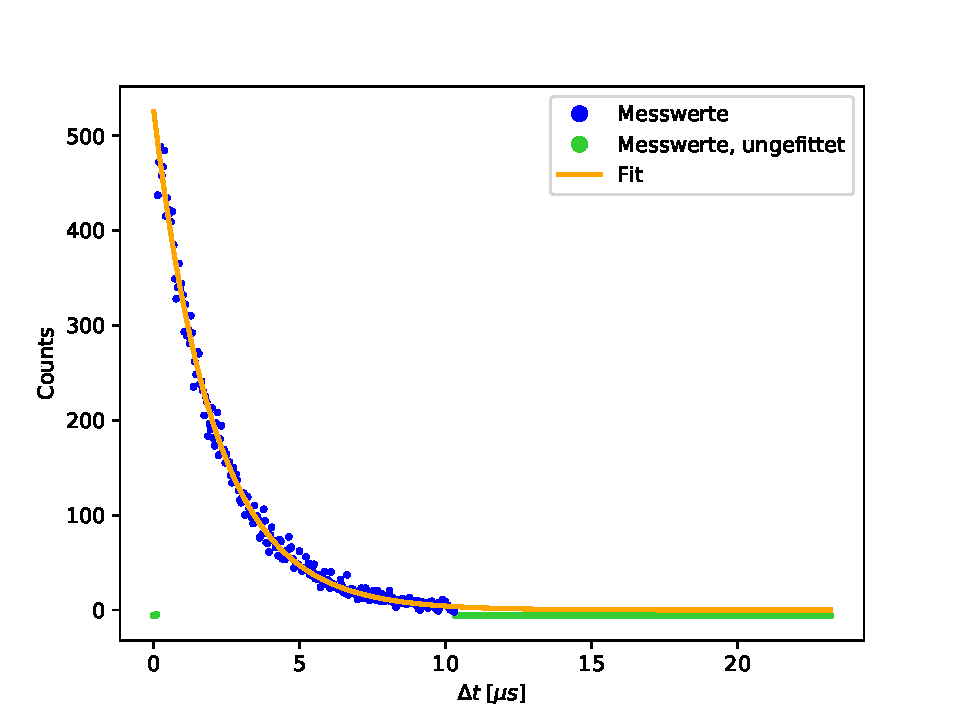
\includegraphics[width = 0.8\textwidth]{plots/Lebenszeit.pdf}
            \caption{Die über 4 Tage aufgenommenen Counts sind gegen die Zeitintervalle vom Start bis zum Stopp der jeweiligen Messung aufgetragen. Aufgrund der Einschränkung durch das gewählte Messintervall werden die grün markierten Messpunkte nicht beachtet.}
            \label{fig:Lebenszeit}
        \end{figure}

        \FloatBarrier

        Über einen Zeitraum von ca. 90,9 Stunden wurden 23944 Myonen-Zerfälle aufgenommen. In \autoref{fig:Lebenszeit} ist wie zu erwarten ein exponentieller Verlauf der Lebenszeit zu erkennen. Zur Bestimmung der Zerfallskonstante $\lambda$ aus dem Zerfallsgesetz \eqref{eqn:Zerfallsgesetz} wird eine Exponentialfunktion an die Messwerte gefittet,
        \begin{equation*}
            f(x) = A \cdot \exp\left(-\lambda t\right) + u
        \end{equation*}
        wobei $u$ der Untergrund während Messung ist. Als Parameter ergeben sich:
        \begin{align*}
            \lambda &= (0,4873 \pm 0,0067) \, \mu\text{s}^{-1} \\
            u &= 7,09 \pm 1,39
        \end{align*}
        Der zuvor berechnete Untergrund von $u_{\text{theo}} \approx 5,81$ ist in der Messunsicherheit enthalten.

        Mit $\lambda$ ergibt sich eine mittlere Myonenlebensdauer von
        \begin{equation*}
            \tau_{\mu} = \frac{1}{\lambda} = (2,052 \pm 0,028) \, \mu\text{s}
        \end{equation*}
        mit einer relativen Messabweichung vom Theoriewert $\tau_{\text{theo}} \approx 2,197 \, \mu$s von:
        \begin{equation*}
            a_{\tau} = \frac{\tau_{\mu} - \tau_{\text{theo}}}{\tau_{\text{theo}}} \approx 6,6 \%
        \end{equation*}


















































